% =============================================================================
\section{Resultados y Experimentos}
% =============================================================================

% ---------------------------------------------------------------------------
\subsection{Configuración experimental}
% ---------------------------------------------------------------------------

Se ejecutaron 30 réplicas de cada escenario usando números aleatorios comunes
(CRN) con semilla base $s_0 = 42$.
Cada réplica modela un día completo de operación (660 minutos).
La correlación observada entre las réplicas pareadas fue $\hat{\rho} = 0{,}552$,
confirmando la eficacia del CRN.

% ---------------------------------------------------------------------------
\subsection{Tabla de resultados}
% ---------------------------------------------------------------------------

La \cref{tab:resultados} presenta la media y el intervalo de confianza al
95\,\% (distribución $t$ de Student con $n-1 = 29$ grados de libertad) para
cada métrica de salida.

\begin{table}[H]
  \centering
  \caption{Resultados de la simulación --- media e IC~95\,\% (30 réplicas, CRN).}
  \label{tab:resultados}
  \setlength{\tabcolsep}{6pt}
  \begin{tabular}{l
                  S[table-format=2.3]
                  @{\;}
                  l
                  S[table-format=2.3]
                  @{\;}
                  l}
    \toprule
    \textbf{Métrica}
      & \multicolumn{2}{c}{\textbf{Escenario A}}
      & \multicolumn{2}{c}{\textbf{Escenario B}} \\
    \cmidrule(lr){2-3}\cmidrule(lr){4-5}
      & {Media} & {IC 95\,\%}
      & {Media} & {IC 95\,\%} \\
    \midrule
    \% clientes $>$ 5 min      & 16.70 & {[13.69,\;19.72]} & 3.10  & {[2.01,\;4.19]}   \\
    Espera media (min)          & 2.185 & {[1.880,\;2.491]} & 0.658 & {[0.566,\;0.750]} \\
    Espera máxima (min)         & 13.46 & {[12.00,\;14.93]} & 7.37  & {[6.51,\;8.22]}   \\
    Longitud media de cola (clientes) & 0.482 & {[0.408,\;0.556]} & 0.146 & {[0.123,\;0.169]} \\
    Utilización media (\%)      & 57.16 & {[55.67,\;58.66]} & 50.16 & {[48.82,\;51.50]} \\
    \bottomrule
  \end{tabular}
\end{table}

Los intervalos de confianza de ambos escenarios no se solapan en ninguna
métrica, lo cual sugiere diferencias sustanciales; la significancia se
verifica formalmente con el test pareado que se reporta a continuación.

La \cref{fig:dashboard} presenta una visión integrada de los cuatro
indicadores principales.

\begin{figure}[H]
  \centering
  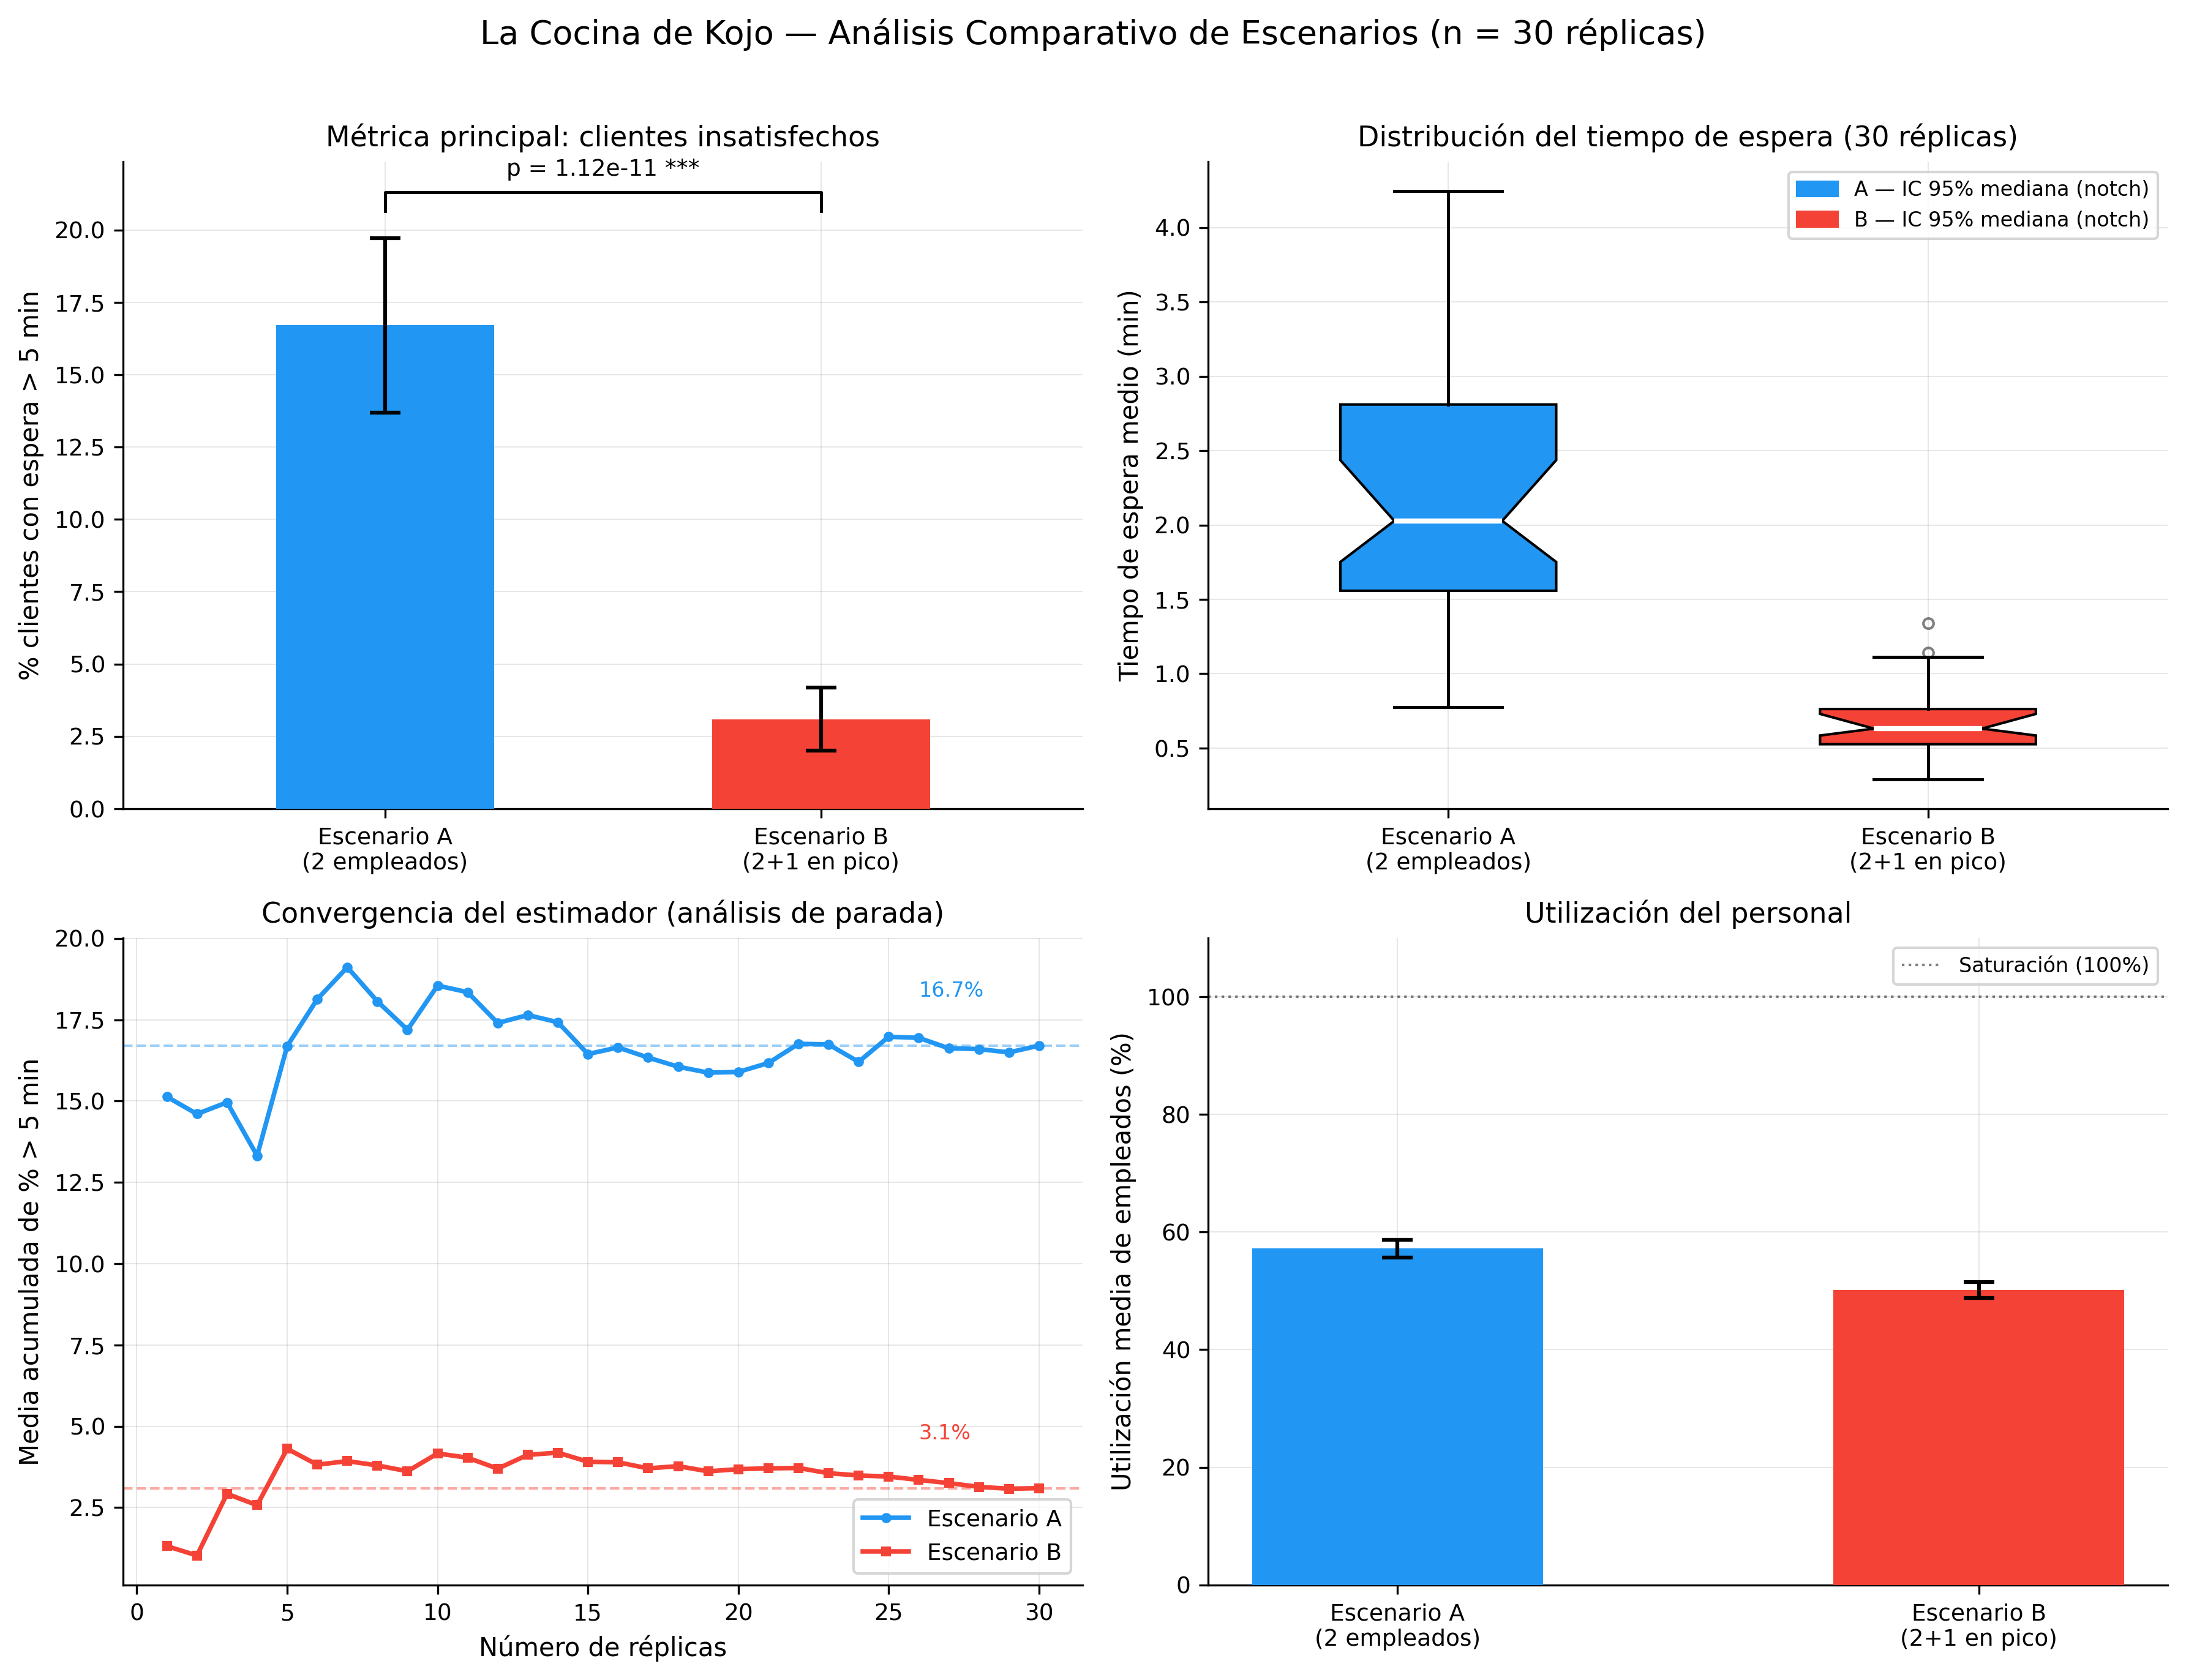
\includegraphics[width=\linewidth]{figures/dashboard.png}
  \caption{Panel comparativo con las cuatro métricas principales.
           Barras de error = IC 95\,\%; notches en box plots = IC 95\,\%
           de la mediana (bootstrap, $B = 5\,000$).}
  \label{fig:dashboard}
\end{figure}

% ---------------------------------------------------------------------------
\subsection{Comparación estadística entre escenarios}
% ---------------------------------------------------------------------------

Se emplea un \textbf{$t$-test pareado} (también llamado test de muestras
relacionadas), ya que las réplicas de A y B están emparejadas por CRN.
El test trabaja sobre las diferencias $D_i = A_i - B_i$:

\[
  H_0: \mu_D = 0
  \qquad \text{vs.} \qquad
  H_1: \mu_D \neq 0,
\]

con estadístico $t = \bar{D} / (S_D / \sqrt{n})$.
Los resultados son:

\begin{center}
\begin{tabular}{ll}
  \toprule
  Diferencia media $\bar{D}$ & $13{,}61$\,\% \\
  IC 95\,\% de $\bar{D}$     & $[11{,}03,\;16{,}18]$\,\% \\
  Estadístico $t$             & $10{,}799$ \\
  $p$-value                   & $1{,}12 \times 10^{-11}$ \\
  Significativo ($\alpha=0{,}05$) & Sí \\
  \bottomrule
\end{tabular}
\end{center}

El intervalo de confianza de la diferencia no contiene el cero.
Se rechaza $H_0$ con un nivel de confianza superior al 99{,}99\,\%:
el tercer empleado reduce significativamente el porcentaje de clientes
insatisfechos.

La \cref{fig:boxplots} muestra la distribución de los tiempos de espera
a través de las 30 réplicas.
Los notches (IC 95\,\% de la mediana) de ambos escenarios no se solapan,
corroborando el test paramétrico con una técnica no paramétrica.

\begin{figure}[H]
  \centering
  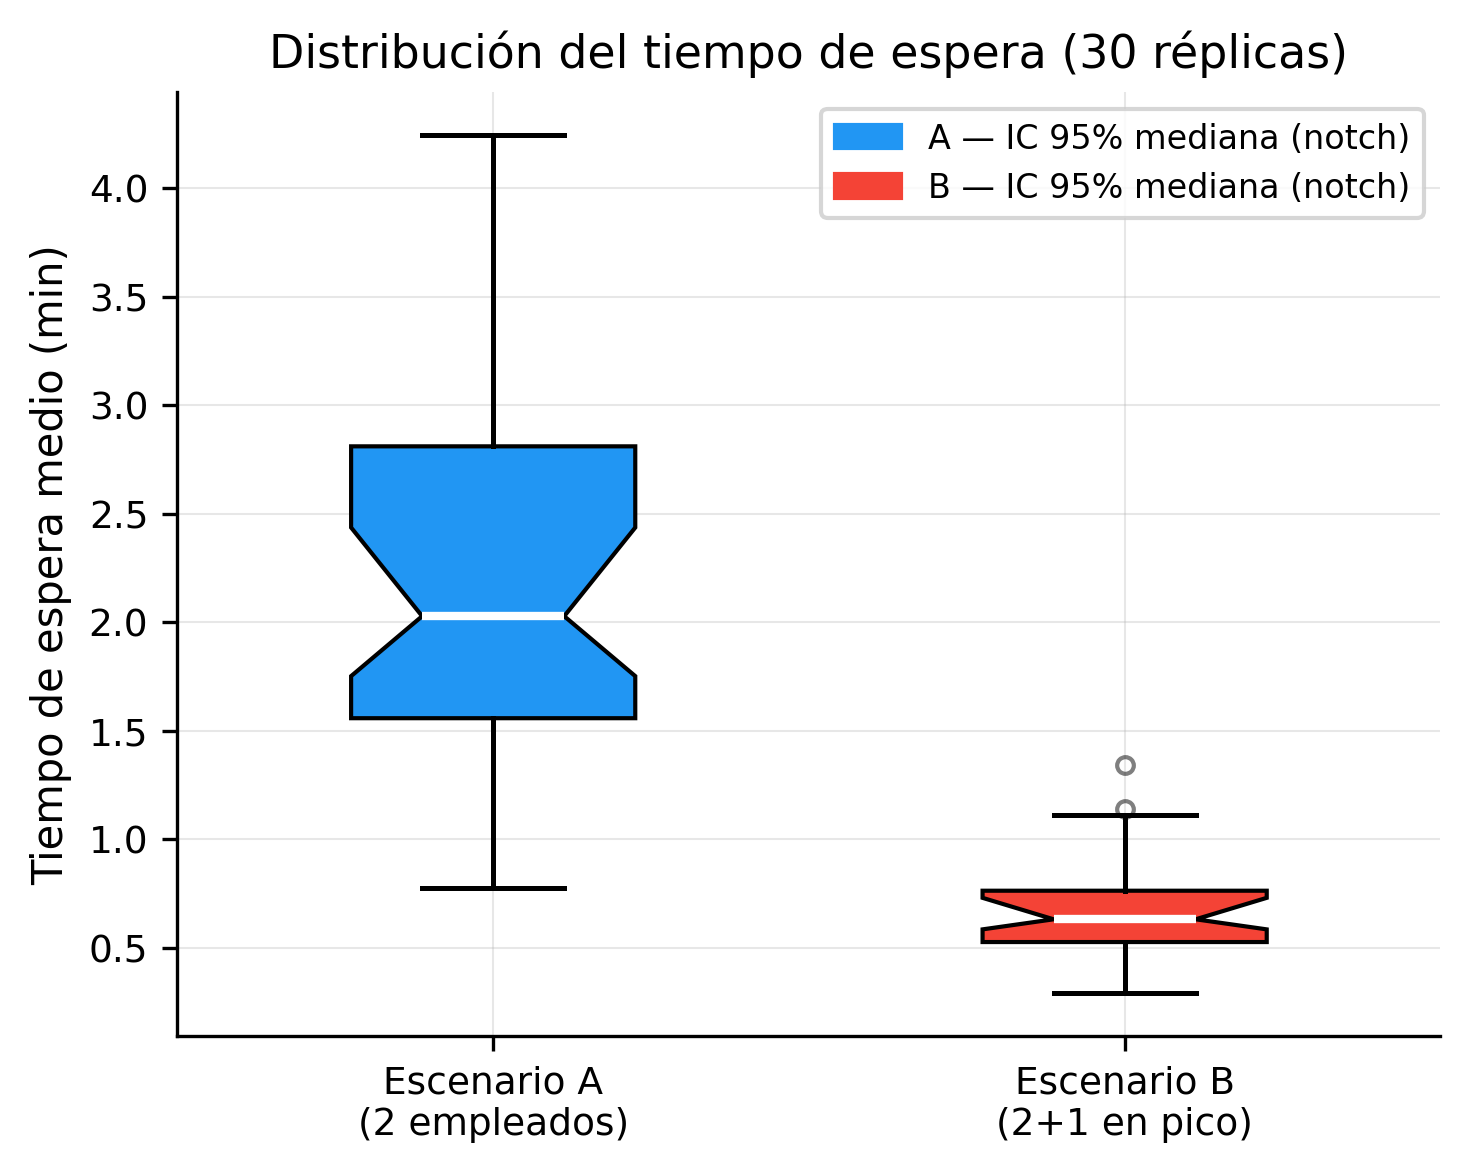
\includegraphics[width=0.7\linewidth]{figures/wait_boxplots.png}
  \caption{Box plots del tiempo de espera medio por réplica.
           Los notches representan el IC 95\,\% de la mediana
           (bootstrap, $B = 5\,000$).}
  \label{fig:boxplots}
\end{figure}

% ---------------------------------------------------------------------------
\subsection{Análisis de parada de la simulación}
\label{sec:parada}
% ---------------------------------------------------------------------------

El criterio de parada de~\citet{curso_temas} establece continuar hasta que
$S/\sqrt{n} < d$.
Equivalentemente, el número mínimo de réplicas para una
precisión relativa $r$ es~\citep{law2015simulation}:
\begin{equation}
  n^* = \left\lceil \left(
    \frac{t_{\alpha/2,\,n-1}\;\hat{S}}{r\;\bar{x}}
  \right)^2 \right\rceil,
  \label{eq:n_star}
\end{equation}
con $r = 0{,}05$ (5\,\% de precisión relativa).

Los resultados de aplicar la~\cref{eq:n_star} son:

\begin{center}
\begin{tabular}{lcccc}
  \toprule
  Escenario & $\bar{x}$ (\%) & $\hat{S}$ (\%) & $n^*$ (5\,\% relativo) & Semi-anchura (\%) \\
  \midrule
  A & 16{,}70 & 8{,}07 & 391  & $3{,}01$ \\
  B &  3{,}10 & 2{,}93 & 1493 & $1{,}09$ \\
  \bottomrule
\end{tabular}
\end{center}

\paragraph{Interpretación.}
El criterio de precisión relativa del 5\,\% no se satisface con 30 réplicas.
Esto se debe a la alta variabilidad intrínseca del indicador: el coeficiente
de variación es $CV_A = 8{,}07 / 16{,}70 \approx 48$\,\% para el Escenario A
y $CV_B = 2{,}93 / 3{,}10 \approx 94$\,\% para el Escenario B.
Un $CV$ tan elevado en el Escenario B es consecuencia de que el porcentaje de
clientes insatisfechos es pequeño (media del 3{,}1\,\%) pero con alta dispersión
entre réplicas: algunos días no se produce ninguna espera larga, mientras que
otros sí.
En estas condiciones, alcanzar una precisión relativa del 5\,\% requeriría del
orden de 400--1500 réplicas.

\paragraph{Precisión absoluta.}
Una forma alternativa de evaluar la suficiencia de las réplicas es mediante la
semi-anchura del IC en términos absolutos.
Con 30 réplicas se obtiene:
\begin{itemize}
  \item Escenario A: IC 95\,\% $= [13{,}69;\;19{,}72]$\,\%, semi-anchura $= 3{,}01$\,\%.
  \item Escenario B: IC 95\,\% $= [2{,}01;\;4{,}19]$\,\%, semi-anchura $= 1{,}09$\,\%.
\end{itemize}
Para la decisión de política de personal, conocer que el Escenario A produce
entre el 13{,}7\,\% y el 19{,}7\,\% de clientes insatisfechos, frente al
2{,}0\,\%--4{,}2\,\% del Escenario B, es más que suficiente.
La diferencia entre ambos intervalos es de varios órdenes de magnitud y no
depende de la estimación puntual exacta.

\paragraph{Suficiencia para la hipótesis principal.}
Aunque la precisión relativa del 5\,\% no se alcanza, el $p$-value de
$1{,}12 \times 10^{-11}$ demuestra que la diferencia entre escenarios es
estadísticamente detectable con garantía absoluta usando 30 réplicas.
El criterio de~\citet{curso_temas} controla la precisión de la \emph{estimación
puntual}; la \emph{detección de diferencias} (objetivo principal del estudio)
requiere potencia estadística, no precisión de estimación, y esa potencia queda
demostrada.
Por tanto, 30 réplicas son suficientes para responder la pregunta de negocio,
aunque se recomendaría aumentarlas si el objetivo fuera reportar el porcentaje
exacto del Escenario B con mayor certeza.

La \cref{fig:convergencia} muestra cómo la media acumulada de cada escenario
se estabiliza alrededor de las réplicas 15--20, confirmando que el estimador
converge dentro del experimento de 30 réplicas.

\begin{figure}[H]
  \centering
  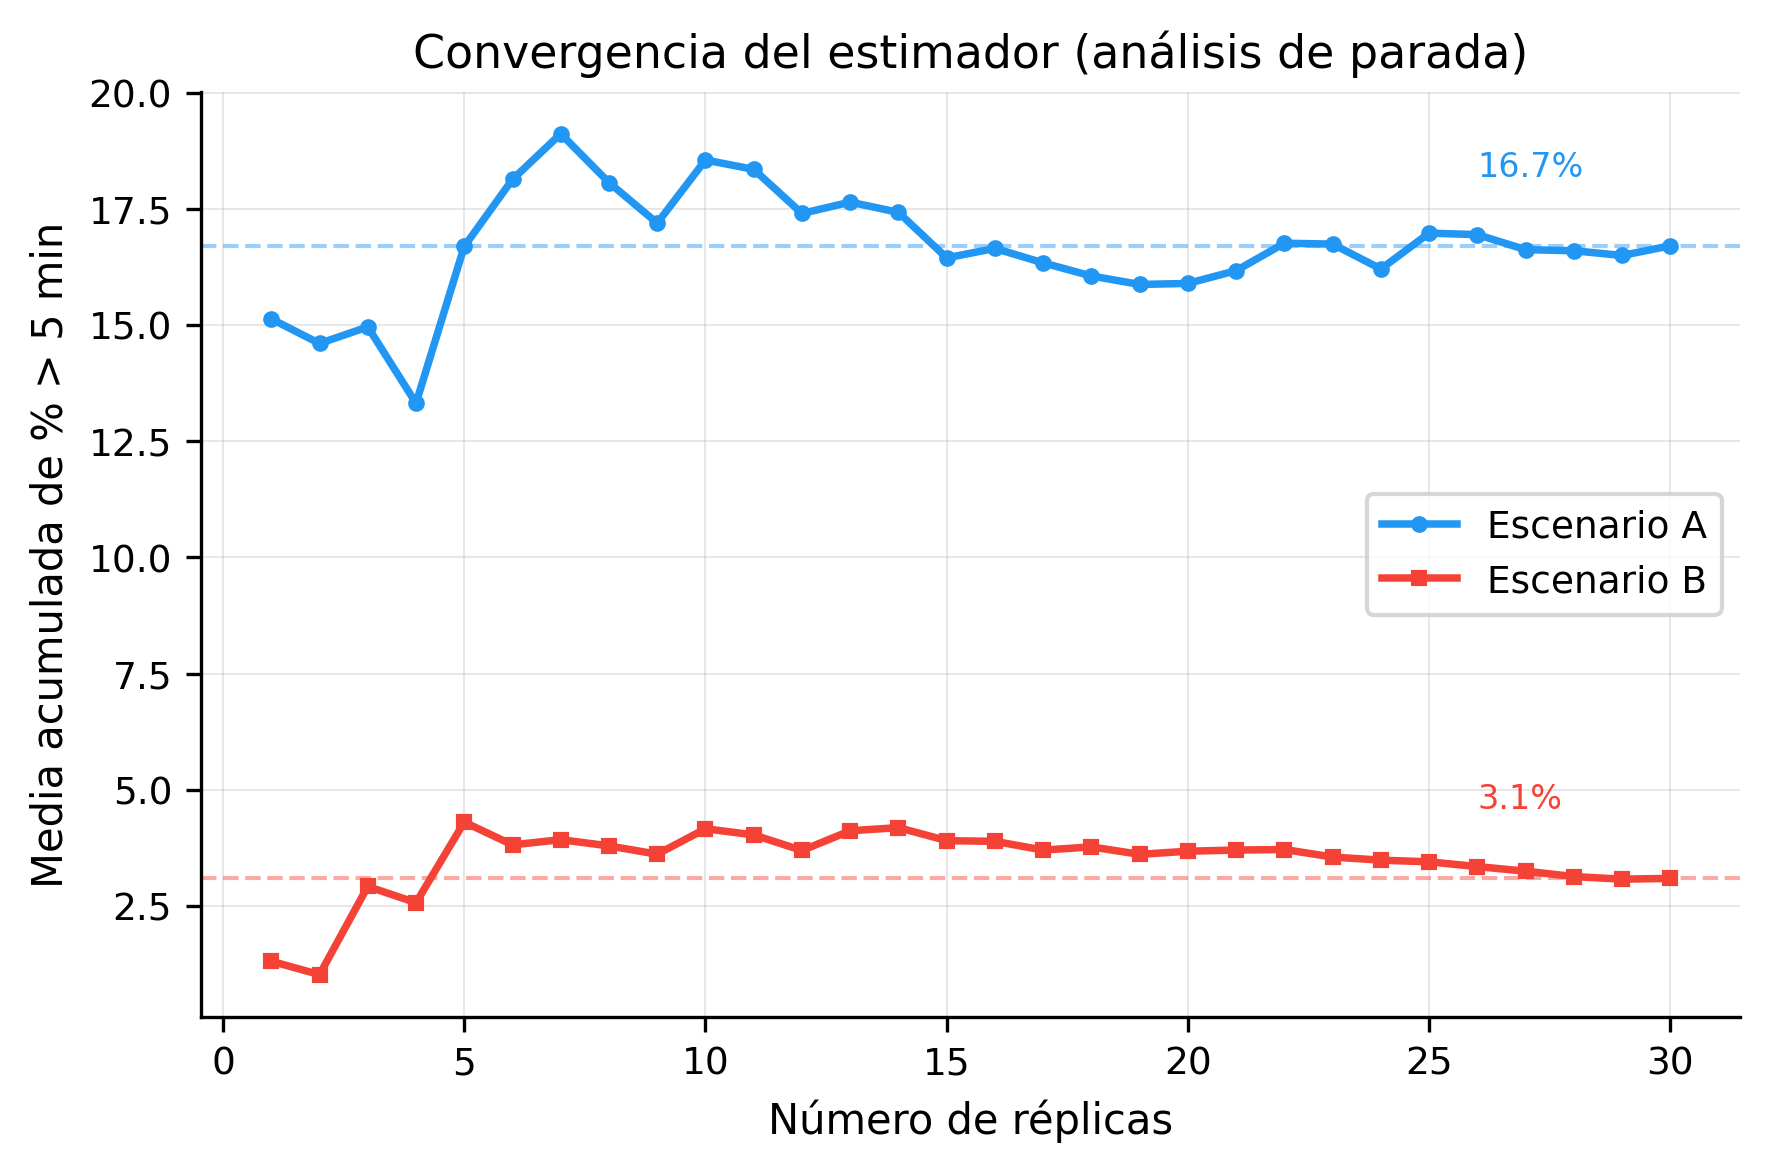
\includegraphics[width=0.85\linewidth]{figures/convergence.png}
  \caption{Convergencia del estimador $\bar{x}_k$ (media acumulada tras $k$
           réplicas). La línea discontinua indica la estimación final.}
  \label{fig:convergencia}
\end{figure}

\begin{figure}[H]
  \centering
  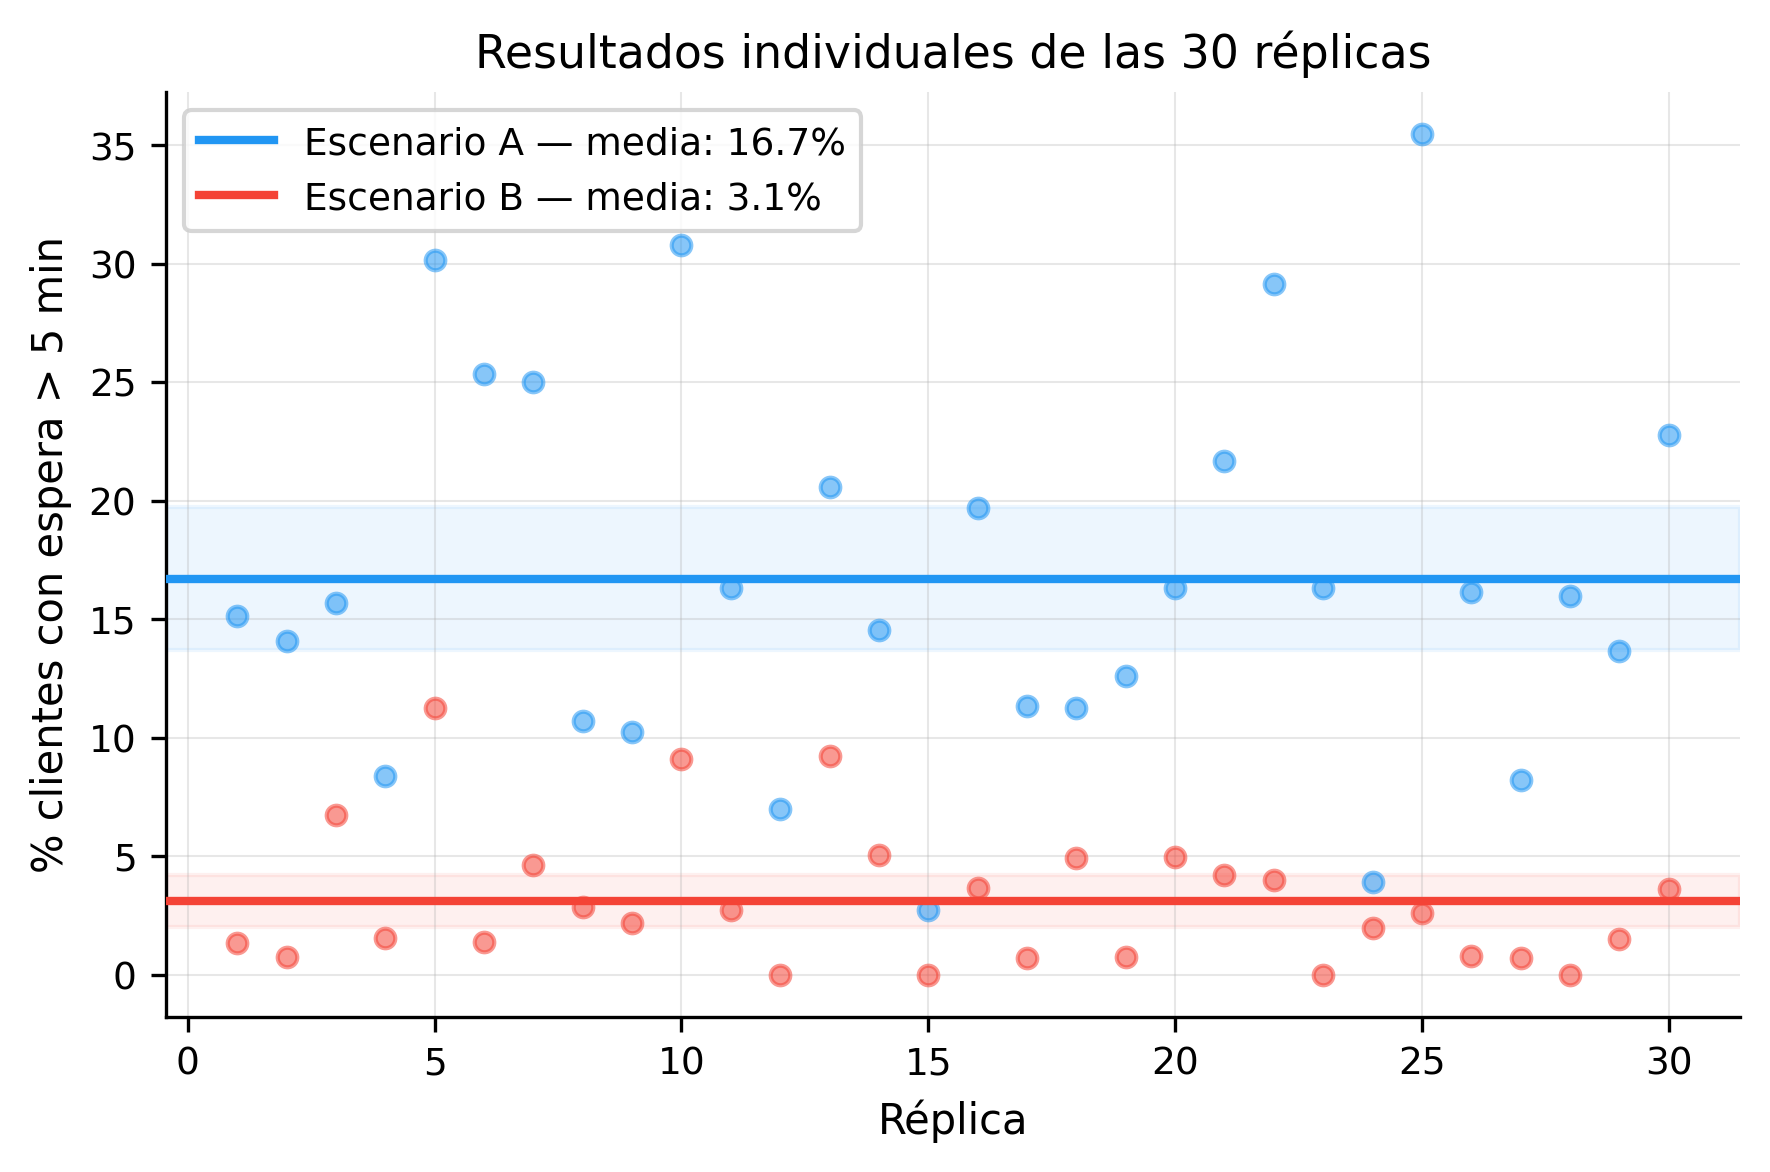
\includegraphics[width=0.85\linewidth]{figures/replication_traces.png}
  \caption{Resultados individuales de las 30 réplicas para cada escenario.
           La línea gruesa es la media; la banda sombreada es el IC~95\,\%.}
  \label{fig:replicas}
\end{figure}

% ---------------------------------------------------------------------------
\subsection{Análisis de sensibilidad}
\label{sec:sensibilidad}
% ---------------------------------------------------------------------------

El enunciado requiere analizar el impacto de la variación de los parámetros
del problema.
Se estudia la sensibilidad de la métrica principal al parámetro más influyente:
la \textbf{tasa de llegadas en hora pico} $\lambda_{\text{peak}}$.

Se ejecutan 10 réplicas por punto para valores
$\lambda_{\text{peak}} \in \{0{,}10,\,0{,}15,\,\ldots,\,0{,}50\}$,
manteniendo constantes el resto de parámetros.

\begin{figure}[H]
  \centering
  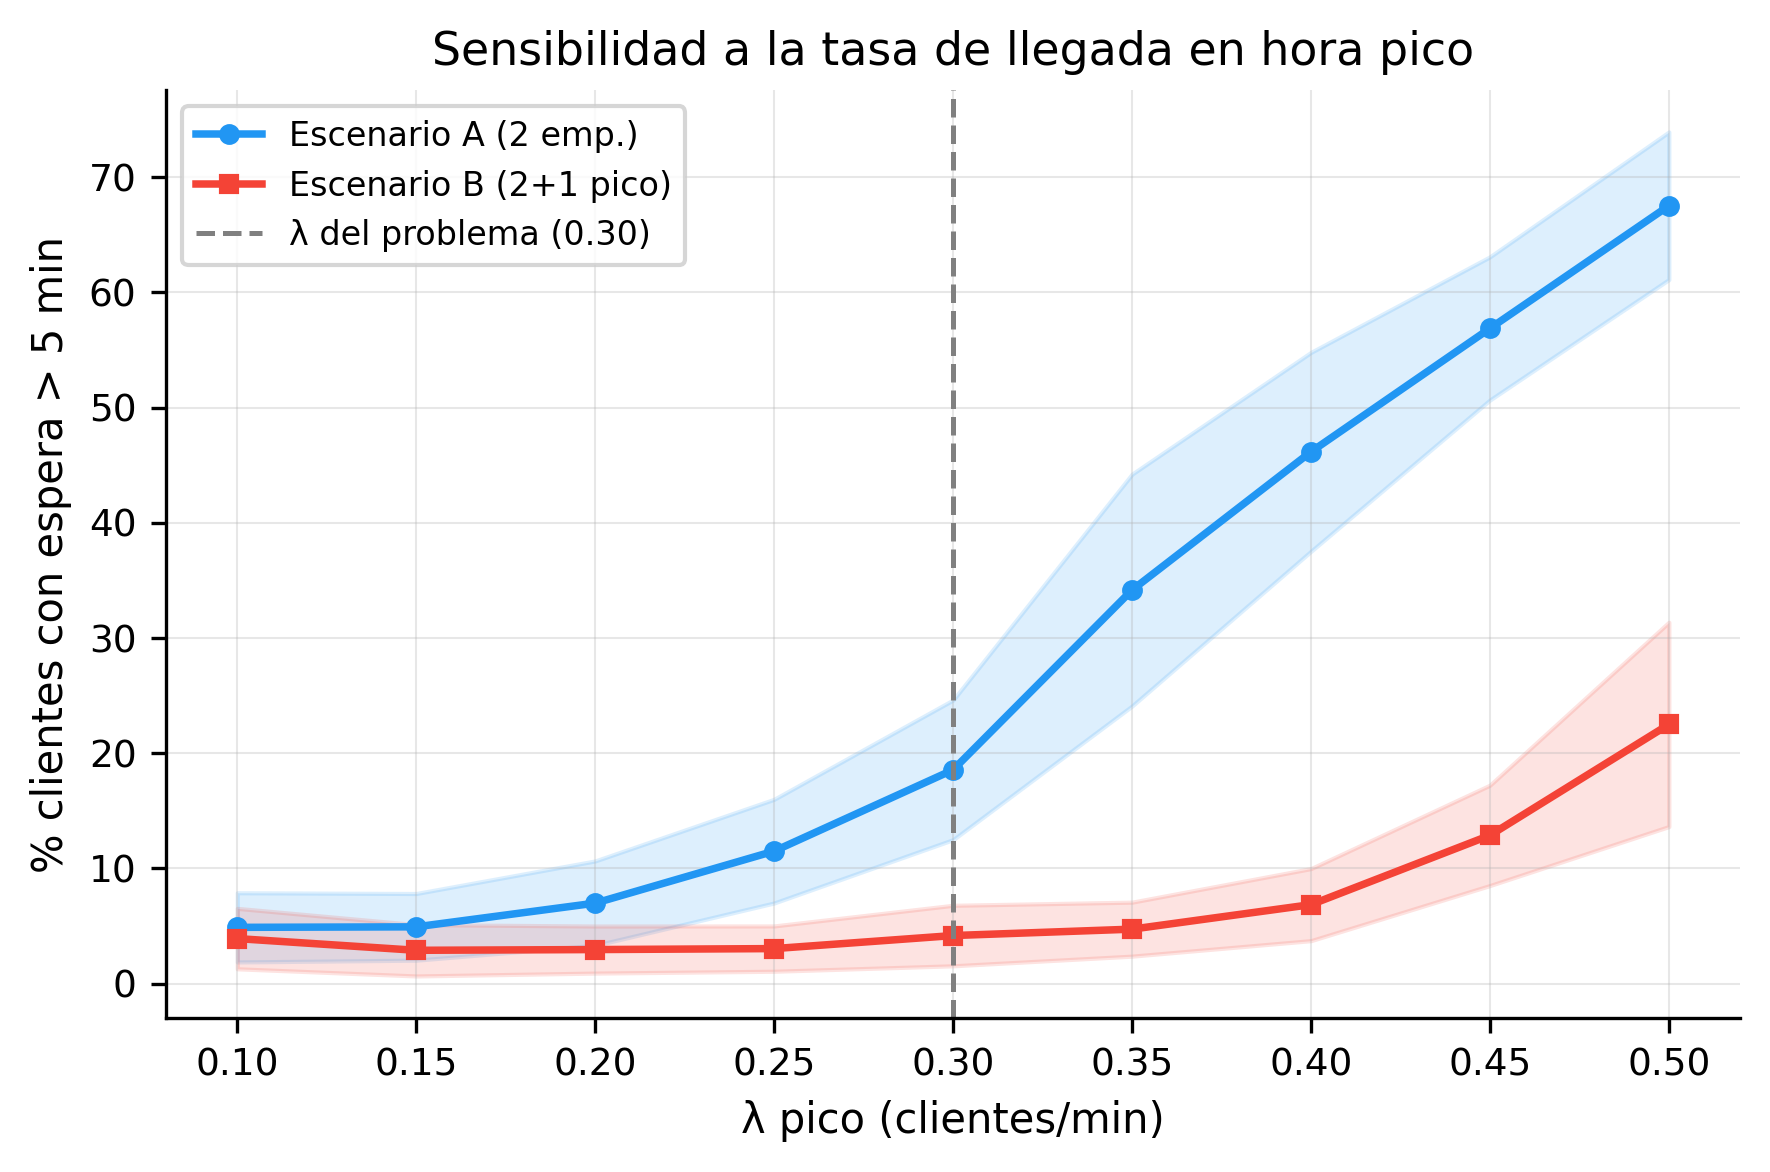
\includegraphics[width=0.85\linewidth]{figures/sensitivity.png}
  \caption{Sensibilidad del \% de clientes con espera $> 5$ min ante
           variaciones en $\lambda_{\text{peak}}$.
           La banda sombreada es el IC 95\,\%.
           La línea discontinua gris marca el valor nominal del problema
           ($\lambda = 0{,}30$).}
  \label{fig:sensibilidad}
\end{figure}

La \cref{fig:sensibilidad} revela varias conclusiones importantes:

\begin{itemize}
  \item Para $\lambda_{\text{peak}} \le 0{,}20$ clientes/min ambos escenarios
    presentan porcentajes de insatisfacción inferiores al 5\,\%;
    la inversión en personal extra no está justificada a esas tasas.
  \item En el valor nominal $\lambda = 0{,}30$, el Escenario B reduce el
    indicador de 16{,}7\,\% a 3{,}1\,\%.
  \item A partir de $\lambda_{\text{peak}} \approx 0{,}42$ el Escenario B
    también comienza a saturarse (supera el 10\,\%),
    indicando que para tasas más altas sería necesario incorporar un cuarto
    empleado durante las horas pico.
\end{itemize}

% ---------------------------------------------------------------------------
\subsection{Sensibilidad a la tasa de llegada fuera de hora pico}
% ---------------------------------------------------------------------------

Se analiza también el impacto de variaciones en la tasa de llegadas fuera de
las horas pico $\lambda_{\text{off-peak}}$.
Se ejecutan 10 réplicas por punto; los valores evaluados son
$\lambda_{\text{off-peak}} \in \{0{,}05;\;0{,}10;\;\ldots;\;0{,}35\}$,
manteniendo $\lambda_{\text{peak}} = 0{,}30$ y el resto de parámetros fijos.

\begin{figure}[H]
  \centering
  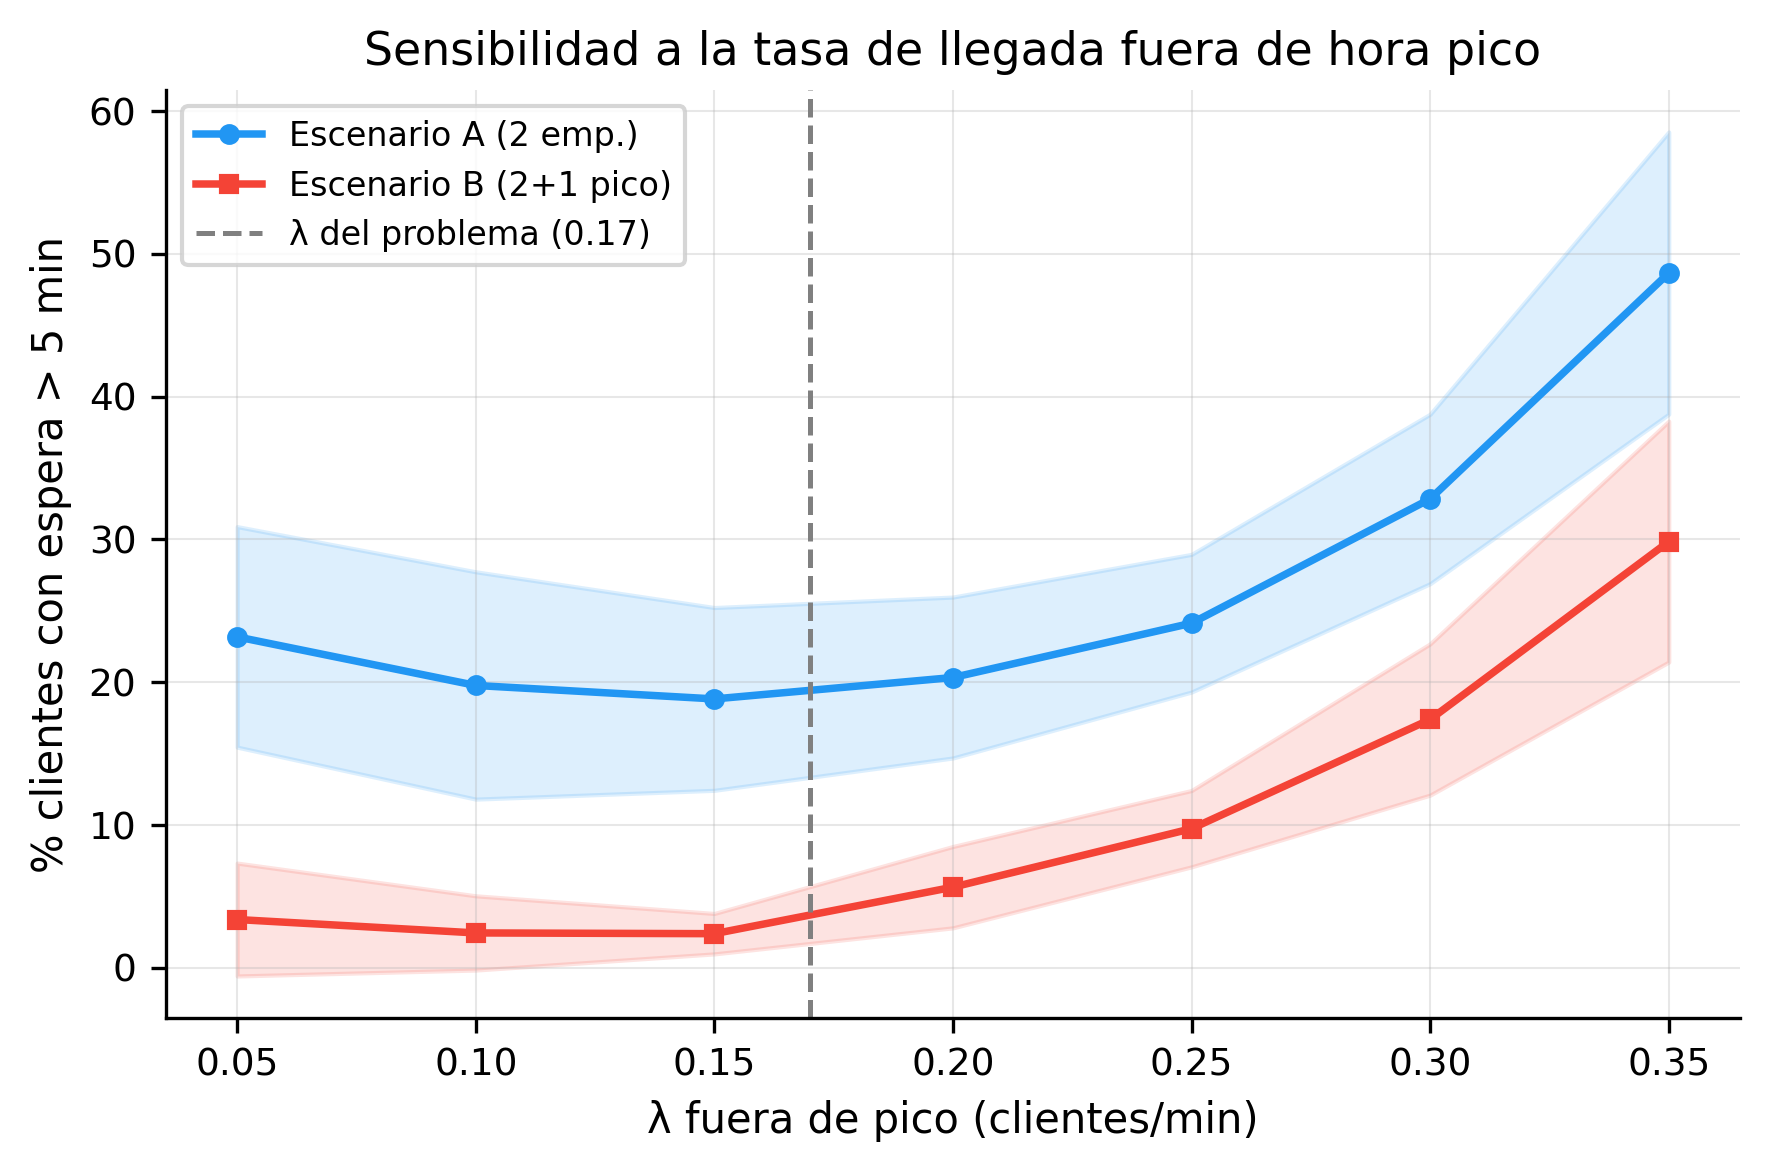
\includegraphics[width=0.85\linewidth]{figures/sensitivity_offpeak.png}
  \caption{Sensibilidad del \% de clientes con espera $> 5$ min ante
           variaciones en $\lambda_{\text{off-peak}}$.
           La banda sombreada es el IC 95\,\%.
           La línea discontinua gris marca el valor nominal
           ($\lambda_{\text{off-peak}} = 0{,}17$).}
  \label{fig:sensibilidad_fuera}
\end{figure}

La \cref{fig:sensibilidad_fuera} muestra que:
\begin{itemize}
  \item La tasa fuera de pico tiene un impacto moderado en comparación con
    $\lambda_{\text{peak}}$: incluso duplicando $\lambda_{\text{off-peak}}$
    desde 0{,}17 hasta 0{,}34, el incremento en el porcentaje de insatisfacción
    es notablemente menor que el producido por variaciones equivalentes en la
    tasa de pico.
  \item El Escenario B mantiene su ventaja frente a A en todo el rango analizado,
    lo que confirma que la recomendación de incorporar un tercer empleado en
    horas pico es robusta ante fluctuaciones en la demanda fuera de pico.
  \item Para $\lambda_{\text{off-peak}} \gtrsim 0{,}30$ clientes/min (valor
    comparable a la tasa de pico), el sistema comienza a saturarse incluso
    fuera de las horas pico, por lo que en ese régimen sería necesario revisar
    la dotación base de empleados.
\end{itemize}
